\documentclass[10pt]{article}
\usepackage[utf8]{inputenc}
\usepackage[T1]{fontenc}
\usepackage[english]{babel}
\usepackage[a4paper,margin=1.65cm]{geometry}
\usepackage{graphicx,booktabs,longtable,array,tabularx,ragged2e,enumitem,caption}
\usepackage[table]{xcolor}
\usepackage{hyperref,xurl,amsmath,tikz}
\usetikzlibrary{arrows.meta,positioning}
\definecolor{HeaderBlue}{HTML}{1F4E79}
\definecolor{LightBlue}{HTML}{EAF2F8}
\hypersetup{colorlinks=true,linkcolor=HeaderBlue,urlcolor=HeaderBlue}
\setlength{\parindent}{0pt}
\setlength{\parskip}{0.32em}
\renewcommand{\arraystretch}{1.14}
\setlength{\tabcolsep}{4pt}
\setlist{leftmargin=*,nosep}
\newcolumntype{Y}{>{\RaggedRight\arraybackslash}X}
\newcolumntype{L}[1]{>{\RaggedRight\arraybackslash}p{#1}}
\captionsetup{font=small,labelfont=bf}
\raggedbottom
\setlength{\emergencystretch}{2em}
\renewcommand{\topfraction}{0.95}
\renewcommand{\bottomfraction}{0.9}
\renewcommand{\textfraction}{0.05}
\renewcommand{\floatpagefraction}{0.85}
\begin{document}
\pagenumbering{gobble}
\begin{titlepage}
\thispagestyle{empty}
\vspace*{0.45cm}
\begin{center}

\includegraphics[width=0.5\textwidth]{assets/Escudo.png}\\[0.35cm]
\rule{\textwidth}{0.6pt}\\[0.6cm]
{\LARGE\textbf{Multi-Hazard Weather Impact Monitoring}}\\[0.3cm]
{\Large Workshop 3: Pipeline Improvements and Gold Layer}\\[0.35cm]
\rule{\textwidth}{0.6pt}\\[0.7cm]
{\large\textbf{Authors}}\\[0.15cm]
{\large\textit{Kevin David Rincon Valencia -- 20232020356}}\\[0.25cm]
{\large\textit{Pablo Garzon Gomez -- 20232020341}}\\[0.7cm]
{\large\textbf{Professor}}\\[0.15cm]
{\large Carlos Andr\'es Sierra}\\[0.7cm]
{\large\textbf{Course}}\\[0.15cm]
{\large Data Analysis Programming -- 2026-II}\\[0.7cm]
{\large Universidad Distrital Francisco Jos\'e de Caldas}\\
{\large Facultad de Ingenier\'ia}\\
{\large Bogot\'a, Colombia}\\
{\large November 2026}
\vfill
\end{center}
\end{titlepage}

\pagenumbering{arabic}
{\Large\bfseries Workshop No. 3: Pipeline Improvements and Gold Layer}

\section{Executive summary and requirement interpretation}
Team 9 implements an Oklahoma weather pipeline with source-aware Silver quality
analysis, PySpark Gold and transactional NWS incremental ingestion. The current
successful Airflow Gold run consolidates 15 checked numeric exports containing
24,972 snapshot rows into \textbf{19,039 unique source records}: 13,561 NOAA
Storm Events records and 5,478 GHCN-Daily measurements for 2021--2025.
It publishes \textbf{650 governance rows and 607 storytelling rows}, with
1,324 distinct NOAA 2021 narratives. Repeated exports are not additional events.
The quality notebook retains the original 13-export review population;
its 22,553 snapshot rows reconcile to the same 19,039 source records.

Saved NWS replay ingests 238 alerts and 700 observations; replaying the bytes
classifies all 938 as unchanged. An explicitly announced live validation on
21 November 2026 returned zero active Oklahoma alerts and 903 KOKC observations.
Reprocessing those captured responses created no additional records or versions.
The current Linux test suites pass 55 tests without skips: 14 Workshop 3,
29 historical/PostGIS and 12 incremental tests. Both notebooks execute without
errors. The 24 November course EDA update is incorporated through DataFrame
profiling, descriptive statistics, SciPy shape measures, IQR/Z-score review,
correlation and two actual HTML profiling reports.
Technical evidence does not establish personal approval or platform submission.

The 2026-II project assigns this milestone incremental ingestion and integration.
The supplied Workshop 3 handout is labelled 2026-I; the team selected it as the
authoritative guide for this delivery [1,2]. Its text, sentiment and keyword
requirements are implemented on genuine NOAA Storm Events narratives where
portable source text exists: registered Oklahoma 2021. VADER lexical tone is
not hazard severity, and this result is not generalized to other years.
The 2010--2025 semester baseline,
broader station inventory, county crosswalk, CHI validation and dashboard remain
separate work. The current historical measurements represent one station.

\section{Pipeline improvements and technical architecture}
\subsection{Before and after}
\begin{tabularx}{\textwidth}{L{2.8cm}YY}
\toprule
Area & Workshop 2 baseline & Workshop 3 change and justification\\
\midrule
Historical inputs & Raw captures, Bronze JSON, validation, database and run-specific Silver Parquet. & Add a Bronze quality-profile verification task and a Silver narrative publication task; mirror checked numerical exports in \path{datalake_silver/}. Raw bytes stay unchanged.\\
Snapshot analysis & Repeated successful exports available as separate snapshots. & Discover every numerical Parquet in \path{datalake_silver/}; require registered hashes or a sidecar; reconcile source/key revisions before statistics.\\
Quality handling & Structural/physical validation and quarantine. & Add source-aware missingness, distribution shape, IQR/Z-score comparison and seasonal context. Review flags do not delete weather extremes.\\
Analytical layer & No executed Gold output. & Local Spark produces typed governance and monthly storytelling datasets in \path{datalake_gold/}, independently reconciled with Pandas.\\
Current ingestion & Incremental CLI was a placeholder. & Add NWS adapters, per-scope state, immutable revisions, quarantine, bounded polling, replay and failure recovery.\\
\bottomrule
\end{tabularx}

\subsection{Implemented paths}
The Airflow practice motivates persistent layer mounts, reusable transformations
outside DAGs and separate acquisition/curation stages [3]. The Workshop 3 handout
specifies local Spark over accumulated Silver files. The revised Bronze
verification and Silver narrative tasks are implemented but have not yet been
executed in Airflow. Local component and Gold runs are identified separately.

\begin{figure}[!htbp]
\centering
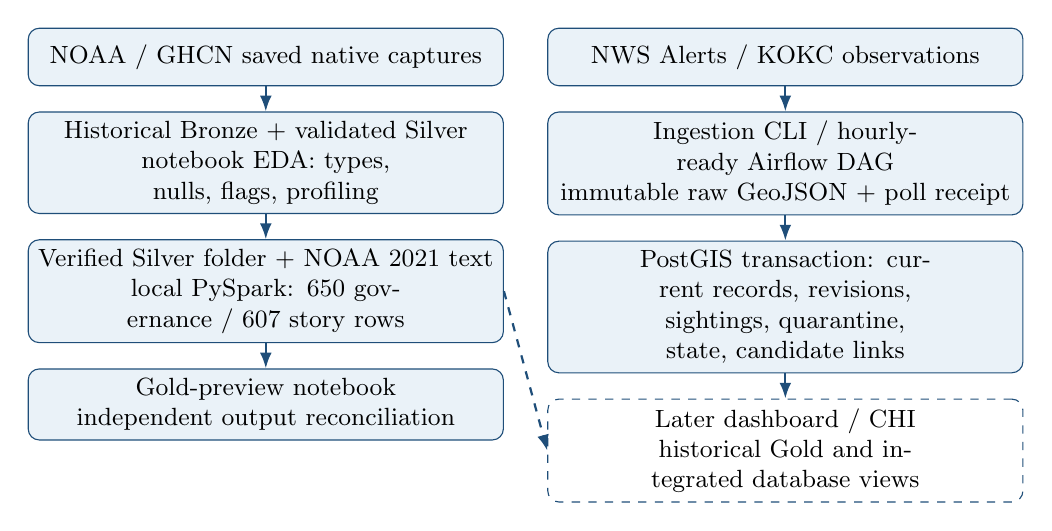
\begin{tikzpicture}[node distance=0.32cm and 0.55cm,
box/.style={draw=HeaderBlue,rounded corners,fill=LightBlue,align=center,text width=5.8cm,minimum height=0.73cm,font=\small},
arr/.style={-{Latex[length=2mm]},thick,draw=HeaderBlue}]
\node[box] (historic) {NOAA / GHCN saved native captures};
\node[box,right=of historic] (nws) {NWS Alerts / KOKC observations};
\node[box,below=of historic] (silver) {Historical Bronze + validated Silver\\notebook EDA: types, nulls, flags, profiling};
\node[box,below=of nws] (raw) {Ingestion CLI / hourly-ready Airflow DAG\\immutable raw GeoJSON + poll receipt};
\node[box,below=of silver] (spark) {Verified Silver folder + NOAA 2021 text\\local PySpark: 650 governance / 607 story rows};
\node[box,below=of raw] (db) {PostGIS transaction: current records, revisions,\\sightings, quarantine, state, candidate links};
\node[box,below=of spark] (notebooks) {Gold-preview notebook\\independent output reconciliation};
\node[box,below=of db,dashed,fill=white] (dash) {Later dashboard / CHI\\historical Gold and integrated database views};
\draw[arr] (historic)--(silver);\draw[arr] (silver)--(spark);\draw[arr] (spark)--(notebooks);
\draw[arr] (nws)--(raw);\draw[arr] (raw)--(db);\draw[arr] (db)--(dash);
\draw[arr,dashed] (spark.east)--(dash.west);
\end{tikzpicture}
\caption{Implemented processing paths; the dashed consumer remains future work.
Editable Mermaid source: \protect\path{workshop_3/architecture.mmd}.}
\end{figure}

The project-level database/view consumer and the handout's Gold-only dashboard
wording remain an explicit specification difference. This report prepares both
traceable contracts without claiming that a final dashboard source decision has
professor approval. NWS records do not silently enter the frozen historical Gold.

\section{Silver data quality findings}
\subsection{Population and source-aware interpretation}
The quality notebook verifies input bytes and schemas before concatenation.
Within one local database history, successful run IDs order observed snapshots.
Copies of the same business key/revision must agree. The latest successful
observed run is selected per source/key; this is not a claim about a global
source revision sequence. Units, station, variable and time grain remain separate.

\begin{longtable}{L{3.0cm}L{5.6cm}L{8.2cm}}
\toprule Finding & Observed evidence & Handling / governance consequence\\\midrule
Repeated exports & 22,553 input rows; 19,039 unique source/key records; 3,514 replay copies. & Reconcile snapshots before aggregation. Report repeated-snapshot fraction and post-selection duplicate-key fraction separately. No independent event inflation.\\
Missing storm point & 7,084/13,561 Storm Events records lack latitude and longitude (52.24\%). & Retain legitimate zone/county records. Report missing-point coverage; do not fabricate point coordinates or geocode every zone to a centroid.\\
Missing storm magnitude & 56.21\% of Storm Events magnitude/value fields are missing. & Count measured records separately; do not replace missing magnitude with zero. Aggregate only compatible type/unit groups.\\
Mixed time grain & All GHCN records have a daily date and no UTC instant; Storm Events use UTC instants and no daily-date field. & Expected source semantics, not universal invalidity. Missingness KPIs explicitly distinguish missing/not applicable.\\
Zero-heavy precipitation & 1,826 daily PRCP values; 78.64\% are zero; all-day Q1=Q3=0. & All-day IQR rule is unavailable. Review positive reported precipitation separately; do not label all positive rain erroneous.\\
Seasonality / extremes & Pooled TMAX/TMIN include seasonal variation; precipitation has a long right tail. & Retain extremes; compare month-specific distributions and proposed IQR/Z-score flags. Statistical rarity is not physical invalidity.\\
QC / schema semantics & Source QC attributes remain available; structural checks cover the 18-field Silver contract. & Report nonempty QC indicators separately. Structural compliance does not certify all meteorological values or assert that every QC flag is a failure.\\
\bottomrule
\end{longtable}

\subsection{Descriptive statistics and outlier review}
Missing measurements are excluded from variable-level moments; sample sizes are
shown. Standard deviation uses $n-1$. Skewness follows the course SciPy calculation;
kurtosis is excess kurtosis (normal reference zero). We use the instructor's
\texttt{scipy.stats.skew()} and \texttt{scipy.stats.kurtosis()} calls and equivalent
Spark moments. No additional estimator comparison is introduced. Values below are
rounded for display; exact results are in \path{evidence/eda_20261124/distribution_review.csv}.

\begin{tabularx}{\textwidth}{Yrrrrrr}
\toprule Population & $n$ & Mean & Median & SD & Skewness & Excess kurtosis\\\midrule
PRCP, all days (mm) & 1,826 & 2.395 & 0.000 & 8.710 & 7.290 & 89.389\\
PRCP $>0$ mm & 390 & 11.215 & 5.100 & 16.023 & 3.690 & 24.867\\
TMAX (degrees C) & 1,826 & 22.946 & 24.400 & 10.084 & -0.617 & -0.062\\
TMIN (degrees C) & 1,826 & 10.171 & 11.100 & 9.748 & -0.420 & -0.715\\
\bottomrule
\end{tabularx}


The proposed review rule is $x<Q_1-1.5\,IQR$ or $x>Q_3+1.5\,IQR$,
only if $IQR>0$. Z-score comparison uses $|x-\bar{x}|/s>3$ only for positive
sample SD. These calculations follow the reviewed class code [9,10].
The slide treatment decision tree asks for context before removal; the classroom
Australian-weather cutoffs are not transferred to Oklahoma as universal rules.

For positive reported PRCP, Q1=1.3 mm, Q3=15.5 mm and IQR=14.2 mm; the upper
review bound is 36.8 mm. IQR flags 25 values versus 6 under Z-score. For all-day
PRCP, IQR is unavailable and Z-score flags 46 values. Pooled TMAX has 14 IQR and
9 Z-score flags; TMIN has 1 and 2, respectively. These populations and rules
are not interchangeable and are not independently validated anomaly detectors.
No value is deleted, winsorized, imputed or relabelled as a confirmed error.

\begin{figure}[!htbp]
\centering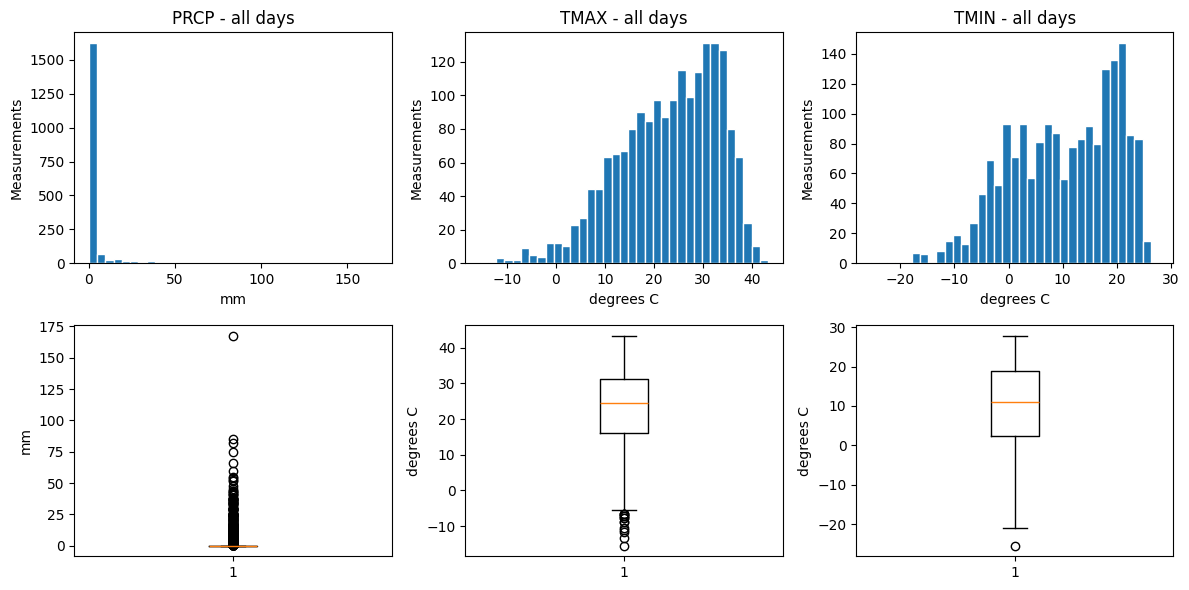
\includegraphics[width=\textwidth]{assets/quality_1.png}
\caption{Actual histogram/boxplot output extracted from the executed Silver
quality notebook. Variable units and zero-heavy precipitation require separate interpretation.}
\end{figure}
\begin{figure}[!htbp]
\centering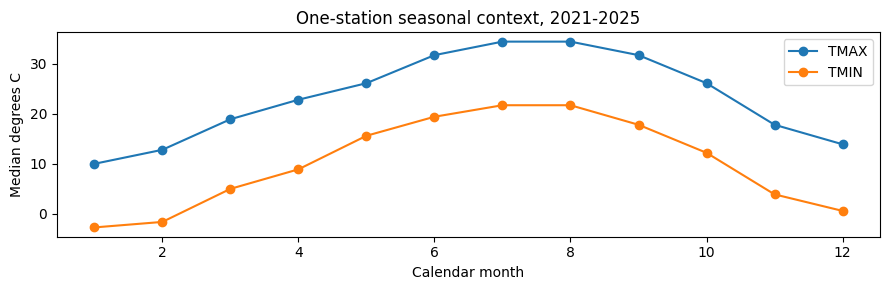
\includegraphics[width=0.9\textwidth]{assets/quality_2.png}
\caption{Actual seasonal-context notebook output. Month-specific comparisons
help separate pooled temperature extremes from normal seasonal variation.}
\end{figure}

\subsection{Course EDA quality gate and automatic profiles}
The updated presentation positions EDA as validation of Silver before Gold [9].
We adapt the instructor's DataFrame inspection, null map, descriptive tables,
SciPy shape calculations, correlation and profiling workflow to the actual
weather sources [10--12]. The notebook reads saved Parquet rather than the
classroom \texttt{weather.json}; no toy-data findings are copied to Oklahoma.
Database identifiers are excluded from weather distribution summaries.

On 1,826 aligned station dates, the selected data has zero missing expected
dates, zero negative PRCP values and zero TMIN$>$TMAX cases. Canonical
source/key duplicates are zero. These are bounded checks, not a certificate of
all dimensions of source accuracy. PRCP has 1,436 zero values (78.64\%);
its zero IQR remains unavailable as a general outlier rule.

Two saved \texttt{ProfileReport} outputs complement the manual audit:
\path{profiling/ghcn_station_quality.html} (1,826 rows/four columns) and
\path{profiling/silver_source_quality.html} (19,039 rows/seven columns).
The second is a reduced projection with source, type, time, point and magnitude
availability; it does not pool incompatible event magnitudes or use numeric IDs
as measured features. Its 501 duplicate-projection warnings do not mean 501
duplicate source keys. Unique dates, zero rainfall and source-inapplicable time
fields are interpreted in context; no record is deleted because of a profile alert.

\begin{figure}[!htbp]
\centering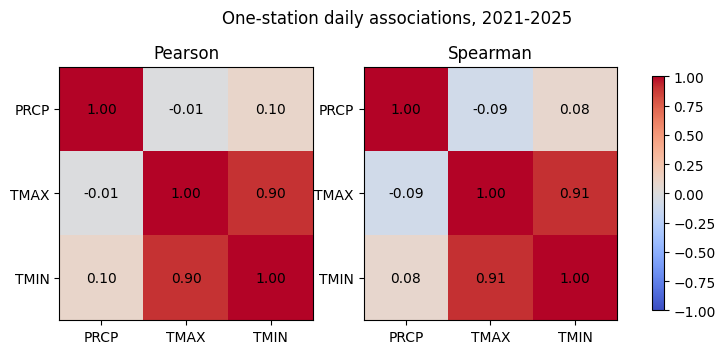
\includegraphics[width=0.9\textwidth]{assets/quality_correlations.png}
\caption{Pearson and Spearman on the same complete daily station records.
The TMAX/TMIN association is descriptive, not causation, a forecast or a reason
to drop either measurement.}
\end{figure}

The class also demonstrates clipping and \texttt{log1p}. We test them only on
an analytical copy. P5--P95 clipping changes 91 PRCP measurements, reducing the
maximum from 167.4 to 16.3 mm and the total from 4,373.7 to 2,819.6 mm.
Because the project monitors weather extremes, clipping is not applied to
Silver or Gold. The \texttt{log1p} view is a distribution experiment, not a
replacement precipitation measurement. No median/KNN imputation, feature
selection or predictive model is added to this delivery.

These findings and decisions are reproducible in
\path{evidence/eda_20261124/}. Academic links, inspected source commit and file
hashes are recorded in \path{evidence/eda_20261124/academic_materials.json}.
The EDA tools run in a separate Python environment; the tested Airflow dependency
contract is unchanged. The earlier delivered revision is retained in a ZIP
archive before this revision under the reported extension.

\section{Governance KPI definitions}
The long-format governance schema uses source, station, population, period,
variable, unit, metric, value, numerator, denominator, method, status and batch ID.
Its grain prevents comparing quantities with different units as one population.
\begin{longtable}{L{4.2cm}L{7.0cm}L{5.6cm}}
\toprule KPI family & Computation & Finding / interpretation\\\midrule
Volume and replay fraction & Count selected records and input snapshots. Replay fraction = (snapshot rows - unique records)/snapshot rows. & Repeated exports can inflate apparent activity. This is a snapshot repetition measure, not source duplication.\\
Canonical duplicate fraction & Repeated source/key groups after deterministic selection, divided by selected source records. & Zero in the verified selection; retained as a preventive invariant.\\
Structural compliance & Count input rows conforming to the implemented required identity, time-grain and typed 18-field contract / checked input rows. & Captures contract drift; does not mean all physical/provider QC tests passed.\\
Source/field null fraction & Null count / records for each source and field. & Separates unmeasured magnitude, missing point and expected daily/instantaneous time semantics.\\
Monthly records & Selected source records per calendar month. & Reveals volume and coverage changes. Counts are records, not exposure-normalized hazard rates.\\
QC indicator fraction & Nonempty provider QC indicator count / applicable measurements. & Supports review without declaring every nonempty indicator an invalid value.\\
Distribution and review flags & Counts, exact quartiles, class shape measures, zero fraction, valid IQR/Z-score flag counts and denominators. & Explains skewness, precipitation zeros and seasonality; unavailable statistics retain explicit status.\\
\bottomrule
\end{longtable}
For fewer than ten values or constant groups, shape statistics remain unavailable,
matching the guard in the instructor's loop. Spark skewness and excess kurtosis
are checked independently against the same SciPy calls used in class. Standard
deviation and Z-score use Pandas sample standard deviation, and quartiles use
linear interpolation. Zero-scale statistics retain an explicit availability
status. Forty numerical checks reconcile, including the zero-IQR PRCP case.

\section{Storytelling aggregations and dashboard narrative}
The narrative is: \emph{describe reported Oklahoma hazards and the airport's
weather context, while showing how coverage and source semantics limit each
comparison}. The key is source/station/month/event-type/unit within a batch.
\begin{tabularx}{\textwidth}{L{4.0cm}YY}
\toprule Existing Workshop 1 story & Implemented Gold support & Boundary / next step\\\midrule
Compare against a seasonal baseline & Station/month PRCP, TMAX and TMIN distributions and monthly summaries. & Formal baseline/current anomaly comparison and 2010--2020 extension remain open.\\
Trace results to source and capture & Source/batch dimensions, input hashes and manifests; Silver retains record-level lineage. & Dashboard drill-down remains future UI work.\\
Review hazards and filter time/type & Monthly reported-event counts by source/type/unit; station time series separately. & County allocation and a current operational panel are not supplied by this historical Gold snapshot.\\
See completeness and freshness & Counts, missing-point and measured-value coverage; incremental status now supplies query times and state age. & Do not display historical batch time as weather freshness. The Gold files themselves are historical.\\
\bottomrule
\end{tabularx}

Storytelling fields include record/measured counts, mean/min/max, observed dates,
missing-point count and PRCP-only precipitation total. The 180 station/month
groups and 427 Storm Events month/type/unit groups reconcile independently.
Temperature and event magnitudes are never summed. Daily dates and UTC event
months are explicit source calendars, not assumed identical accumulation windows.

The first dashboard direction is descriptive (what was recorded) and exploratory
diagnostic (what accompanies a peak). Associations do not establish causes.
Predictive models and prescriptive emergency advice are absent; CHI will remain
a monitoring indicator unless separately validated. Each application must select
one committed analytical batch, rather than adding every dated Gold snapshot.

\section{PySpark implementation and actual Gold results}
The custom Airflow image includes Python 3.12.8, PySpark 3.5.7, Java 17,
Pandas 2.1.4 and PyArrow 18.1.0. The Spark session uses \texttt{local[2]}, a 1 GiB
driver, two shuffle partitions and UTC. It disables Spark UI and does not use
Spark Connect or Pandas-on-Spark. This is a bounded local run, not a scale benchmark.

\path{airflow/dags/gold_processing_dag.py} defines one TaskFlow task,
\texttt{summarize\_silver}, weekly Monday 06:00 UTC, with one active run,
\texttt{catchup=False}, a 20-minute timeout and one retry after 30 seconds.
The registered historical inputs are already materialized; their presence,
hashes and schemas are verified rather than adding a time-window sensor that
could select unrelated files. A weekly schedule is configured; the evidenced
run was manually triggered, not a claim of a week's scheduled operation.

Processing steps are: verify register/config/code/input hashes; read every checked
Parquet path in the Silver folder as one Spark DataFrame; enforce the common schema; reject conflicting
same-key/revision copies; select the latest successful local snapshot; compute
DataFrame/SQL aggregates; write both typed outputs; read back; and atomically
publish one batch manifest. Spark supports this multi-file Parquet pattern [6].

The first real run failed because Hadoop attempted POSIX chmod on the Windows
bind mount. The corrected implementation writes Spark part directories on Linux
\texttt{/tmp}, copies finished files to host staging without changing permissions,
verifies them, then publishes both together. The failed-run and permission-error
receipts are retained; the successful run is not substituted for the failure.

Current successful DAG run: \texttt{w3\_runtime\_gold\_20261125T000455},
24 November America/Bogota (25 November, 00:04--00:06 UTC), first attempt.
It implements \texttt{weather-gold-v2-course-eda}: 650 governance and 607
storytelling rows, including the instructor-aligned shape metrics. All 15 checked
numeric files and two checked text exports were read from the Silver folders.
The 2,648 text snapshot rows reconcile to 1,324 unique narratives, rather than
doubling their counts. Independent Pandas/SciPy comparison verifies 40 numerical
statistics, 180 station/month groups, 427 event groups and narrative/tone totals.

Actual output copies and the original manifest are in
\path{samples/eda_20261124/}; the successful task receipt and test fingerprints
are under \path{evidence/eda_20261124/runtime/}. Earlier 625-row and local
650-row outputs remain historical. The revised Bronze/Silver tasks were also
successfully exercised in the 23 November Docker verification; unchanged replay
preserved canonical records and revisions. All application DAGs are left paused.

\begin{figure}[!htbp]
\centering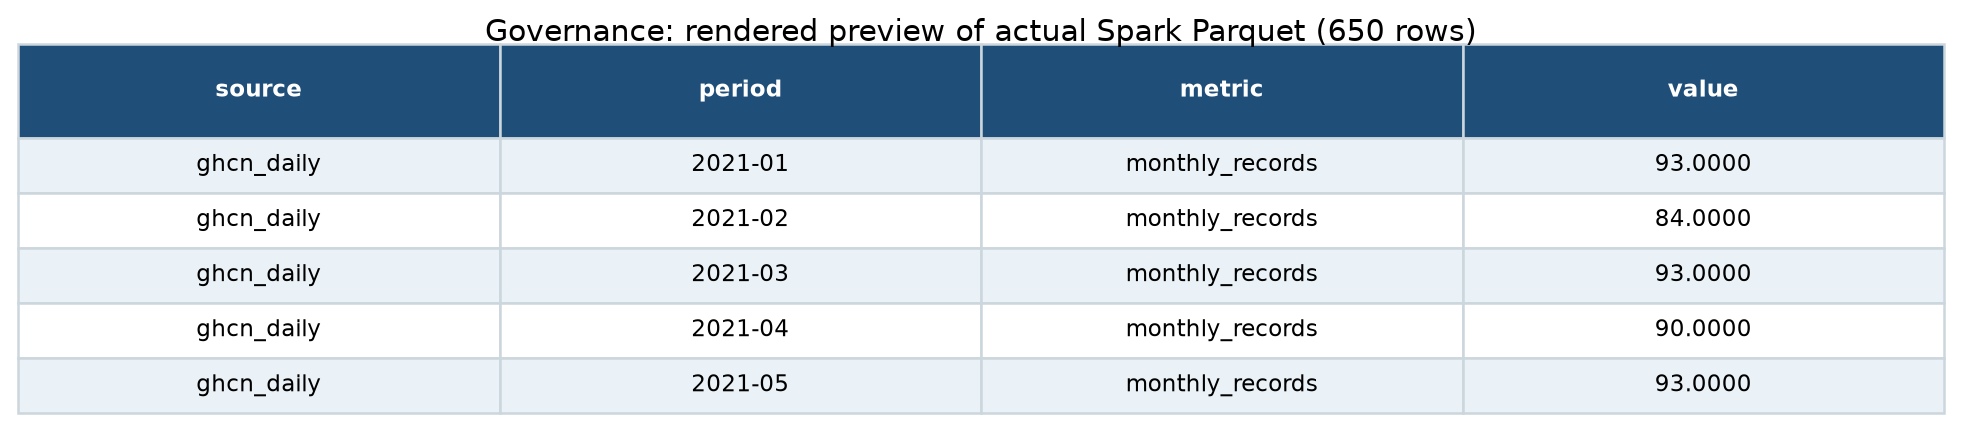
\includegraphics[width=\textwidth]{assets/governance_preview.png}
\caption{Rendered contents of the actual governance Parquet sample. This is a
file-derived table image, not an Airflow browser screenshot. Exact rows are also
provided in \protect\path{samples/gold/governance_preview.csv}.}
\end{figure}
\begin{figure}[!htbp]
\centering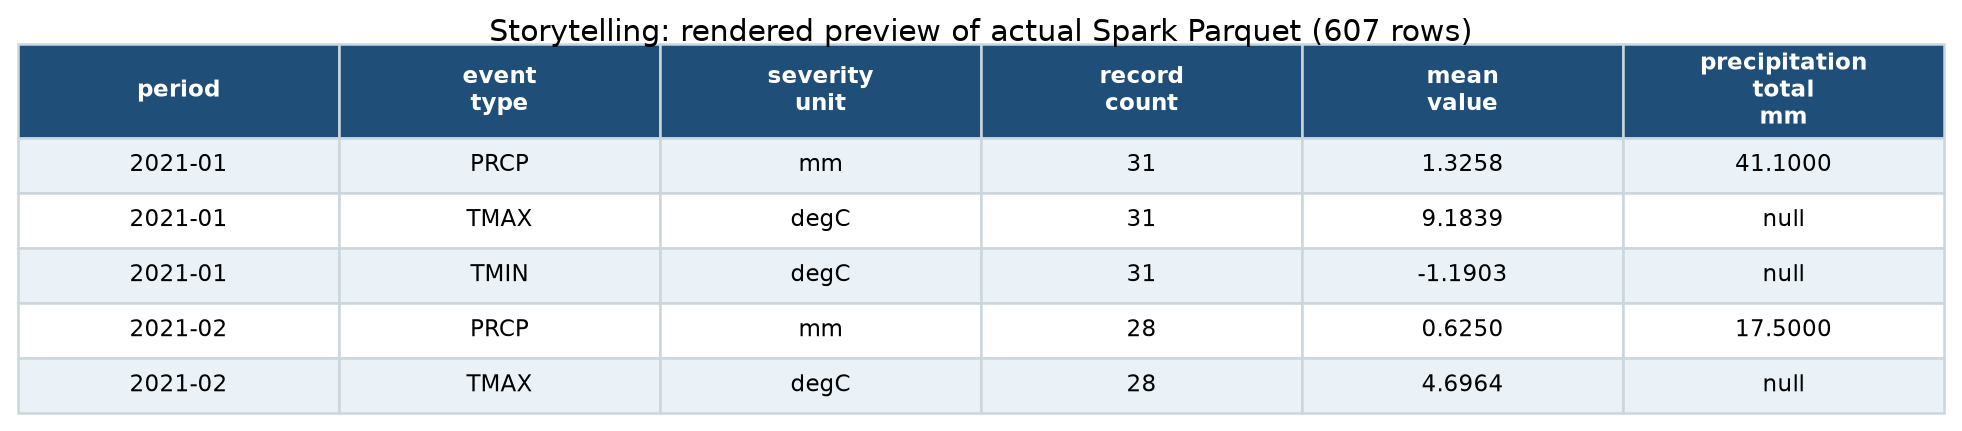
\includegraphics[width=\textwidth]{assets/storytelling_preview.png}
\caption{Rendered contents of the actual storytelling Parquet sample. Displayed
decimals are rounded; the Parquet and CSV retain stored values. Null precipitation
totals for temperatures are deliberate.}
\end{figure}

\subsection{Narrative quality, sentiment and keywords}
The registered NOAA Oklahoma 2021 CSV contains 1,324 rows. Selection uses
\texttt{EVENT\_NARRATIVE} for 632 rows and falls back to
\texttt{EPISODE\_NARRATIVE} for 692; every selected text is nonempty. Original
text remains in the checked Silver sidecar. Its length has mean 280.53,
median 177, minimum 13 and maximum 1,914 characters. Tokens are lowercased
after HTML, URL and mention cleanup; source identity and text-field provenance
are retained. VADER 3.3.2 scores original English text with compound thresholds
$\geq0.05$ positive and $\leq-0.05$ negative [8]. The observed labels are
445 positive, 456 neutral and 423 negative. Gold exposes annual narrative
coverage and length statistics, and monthly/type sentiment counts, mean score
and frequent keywords. These are lexical descriptions of provider narratives,
not weather severity, public opinion, causal explanation or validated accuracy.
The other years have no portable narrative Silver in this delivery, so their
text metrics are marked unavailable, not zero. No live weather call was made.

\begin{figure}[!htbp]
\centering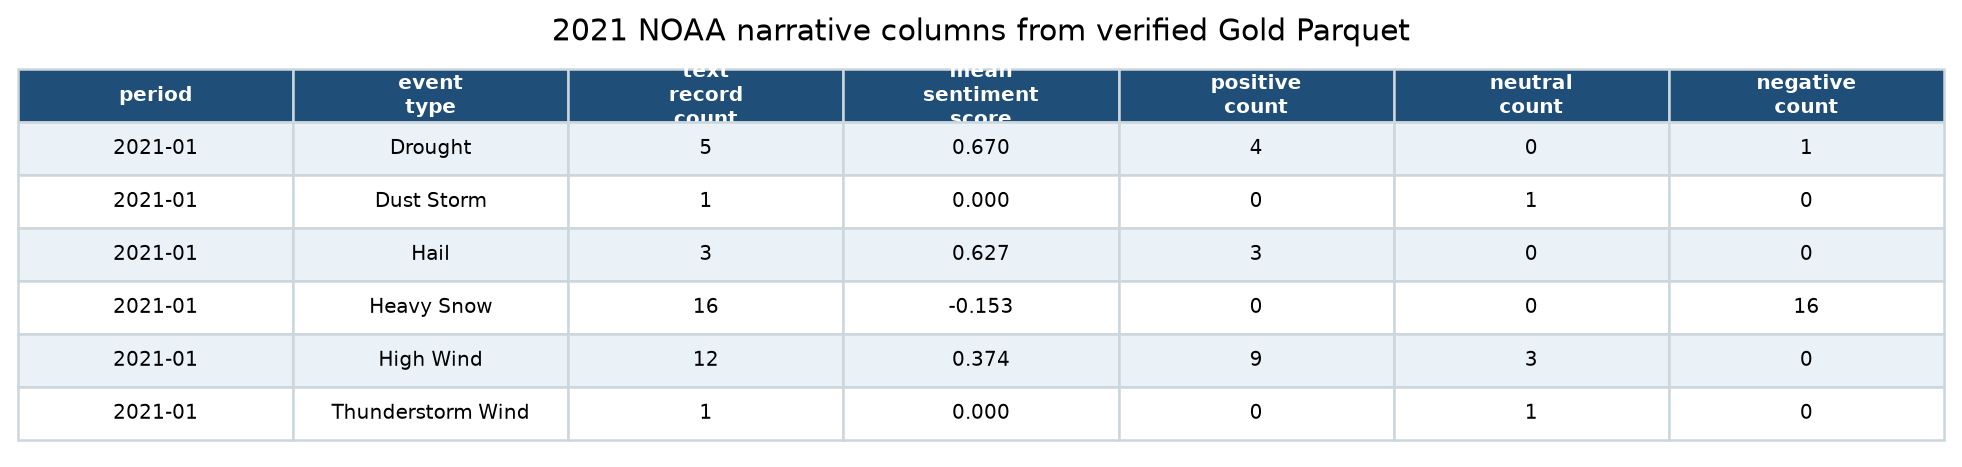
\includegraphics[width=\textwidth]{assets/text_preview.png}
\caption{Rows rendered from the verified Airflow Gold storytelling Parquet.
The underlying sample and exact CSV are under \protect\path{samples/gold/}.}
\end{figure}

\section{Incremental ingestion, state and integration}
\subsection{Source handling and failure recovery}
The CLI now supports incremental replay or an explicit live source. Migration
005 adds poll receipts, current records, immutable revisions, sightings,
quarantine, per-source/namespace/scope state and versioned candidate links.
Replay, test and live namespaces are separate. The integrated operational view
combines historical records and live NWS records, excluding replay/test data.

Every response body is content-addressed under \path{data/raw/}; the poll receipt
records request URL, retrieval timestamp and SHA-256. Feature identity and sorted
content hash distinguish new, unchanged and changed records. Changed source IDs
retain their earlier raw/normalized revisions; unchanged replays add sightings
but no revision. Provider fields and QC codes remain traceable. Wind km/h is
converted to m/s, supported temperatures to degrees C, and precipitation in metres
to millimetres. Unsupported units remain explicit with no invented converted value.

An alerts watermark is the \textbf{timestamp of the last successful complete
query}, not a provider record cursor. Record-level sent/effective/onset/expiry
times are preserved independently. Missing an ID in an active snapshot does not
delete or silently cancel its stored history. Alert lifecycle fields remain source
attributes; current validity must be evaluated using them and poll freshness.

KOKC state uses a one-hour overlap after successful queries and a full seven-day
reconciliation at least every 24 hours. An outage beyond source retention is
flagged in the poll window receipt; the API is not claimed to recover an archive.
The hourly interval, overlap and reconciliation are team policy. NWS documents
seven-day observation retention, required identifying User-Agent, caching and a
nonpublic rate limit [7]. Requests use bounded retries/backoff, timeouts and
Retry-After. Pagination must remain on the trusted HTTPS NWS host and terminate;
cycles, incomplete chains or page limits fail instead of advancing state.

The database transaction commits record changes, versions, sightings, rejects,
metrics and state together. Invalid features are quarantined; rejected or
incomplete polls do not advance the coverage watermark. Failed transactions
roll back changes and retain a separate failure receipt. Advisory locks serialize
source/scope writes; older queries cannot overwrite newer committed snapshots.

The incremental DAG has separate alerts/station tasks, a 15-minute task timeout,
two retries and exponential delay. It was successfully run in replay mode as
\texttt{w3\_nws\_replay\_20261121T151137}; both source tasks and candidate grouping succeeded on first attempt.
An earlier automatic run without explicit mode was blocked before network access
and cancelled; its evidence is retained. The corrected DAG has no automatic
schedule until \texttt{NWS\_POLL\_MODE=live}; hourly scheduling is then enabled.
It was left paused after verification. No ongoing operational service is claimed.

\subsection{Saved replay and announced live validation}
\begin{tabularx}{\textwidth}{YrrrrY}
\toprule Input / pass & Read & New & Changed & Unchanged & Coverage\\\midrule
Saved alerts, first pass & 238 & 238 & 0 & 0 & Complete observed two-page chain.\\
Saved KOKC, first pass & 700 & 700 & 0 & 0 & Partial, non-contiguous snapshots; no coverage watermark.\\
Saved alerts, second pass & 238 & 0 & 0 & 238 & Same bytes, no new revisions.\\
Saved KOKC, second pass & 700 & 0 & 0 & 700 & Same partial-coverage limitation.\\
Live active OK alerts & 0 & 0 & 0 & 0 & Valid empty complete response.\\
Live KOKC, complete query & 903 & 903 & 0 & 0 & Complete returned pagination chain.\\
Captured live KOKC, replay & 903 & 0 & 0 & 903 & No second HTTP query.\\
\bottomrule
\end{tabularx}

The live queries began at 15:05:04 and 15:05:05 UTC on 21 November 2026.
The KOKC request used an explicit seven-day start/end interval. Complete returned
pagination does not prove one observation exists for every expected timestamp or
that delayed provider data will never be revised. Exact URLs, page hashes,
captures and state are in \path{evidence/incremental_live.json}. Small committed
excerpts are explicitly parsed derivatives; original HTTP bytes remain in ignored
raw storage. None of these records is added to the historical Gold statistics.
An offline boundary audit finds 902 returned observations inside the requested
interval and one preceding its start; none follows the requested end. All 903
are preserved. This observed discrepancy is documented in
\path{evidence/nws_window_review.json}; its cause is unverified, and later
analyses must apply explicit timestamp filters rather than assume request bounds.

\subsection{Candidate relationships and uncertainty}
Rule \texttt{nws\_polygon\_validity\_v1} selects one closest observation per alert
whose station point is covered by the alert polygon and whose timestamp lies in
the effective/expiry interval. It stores rule version, both source IDs, content
hashes, temporal/spatial evidence and \texttt{candidate\_not\_confirmed} status.
Missing polygons receive no invented county-name or nearest-centroid fallback.

The saved replay produces \textbf{five intra-NWS temporal/spatial associations}.
They are not independent-source matches, independent weather events, verified
impacts or a match-accuracy evaluation. The live query produces zero candidates
because no active alerts were returned. The five prior Workshop 1 NOAA/GHCN wind
candidate rows are indexed as reused historical context, not newly discovered
Workshop 3 matches; daily peak timing and common reporting lineage remain caveats.
No current Storm Events/GHCN coincidence was validated across the 2026 live window.
Reviewed county allocation and quantitative match precision/recall remain open.

\section{Verification, reproducibility and handoff}
\begin{tabularx}{\textwidth}{L{4.2cm}YY}
\toprule Check & Result & Traceable evidence\\\midrule
Workshop 3 / Spark & 14 passed in Linux Docker, including course-moment, folder/text and snapshot-reconciliation guards. & \path{evidence/eda_20261124/runtime/linux_tests.json}\\
Historical/PostGIS & 29 passed; no PostgreSQL cases skipped. & Same current Linux test receipt.\\
Incremental fixtures & 12 passed; revisions, state, recovery and candidate status. Synthetic fixtures are not weather observations. & Same current Linux test receipt.\\
Gold comparison & 40 numerical statistics; 180 station and 427 event groups; 1,324 unique narratives reconcile. & \path{evidence/eda_20261124/gold_reconciliation.json}\\
Notebooks / profiles & Quality: 16 code cells; Gold preview: 6; zero errors, fresh isolated kernels. Two HTML profiles generated. & Current execution receipts and profile hashes under \path{evidence/eda_20261124/}.\\
Airflow & Current 650/607 Gold run succeeded; actual revised Bronze/Silver success and unchanged replay retained. & Current Gold receipt plus \path{evidence/runtime_20261123/}.\\
\bottomrule
\end{tabularx}

The review package includes this PDF, its editable LaTeX/assets, two executed
notebooks, actual governance/storytelling Parquet samples, code, configuration,
SQL migration and an evidence register. Paths and commands are documented in
\path{deliveries/03-workshop-3/DEMO_GUIDE.md}. The committed Silver reproduction
ZIP restores all 13 reviewed input files offline, byte for byte, without replacing
different existing files. A clean temporary restore and unchanged second restore
verified all 13 hashes. Source response samples and test
fixtures remain clearly distinguished. Apply migrations through the checksummed
runner; do not edit already applied SQL. Rebuild/recreate the configured image
when runtime/environment changes, without deleting the persistent database volume.

A controlled PostgreSQL restart preserved row counts and hashes of incremental
state, records, revisions and candidate links. The historical count remained
19,039; the operational integrated view contains 19,942 unique source/key rows
(historical plus 903 live observations), excluding replay/test records. Exact
before/after evidence is in \path{evidence/incremental_restart.json} and
\path{evidence/incremental_database_audit.json}.

\textbf{Remaining boundaries.} Kevin and Pablo must review the report, mapping
and runtime decisions before integration; no new personal approval is recorded.
The reviewed classroom EDA methods are now explicitly implemented. County
crosswalk, broader station/year coverage, match evaluation,
CHI and dashboard are not declared resolved. The current branch is
\texttt{feat/workshop-3-quality-gold}; commit, push, merge and platform submission
remain student actions. No submission date or delivery acceptance is invented.

\section*{References}
{\small
\begin{enumerate}[label={[\arabic*]}]
\item Course project, Semester 2026-II.
\href{https://github.com/EngAndres/ud-public/blob/main/courses/data-analysis-programming/project/CourseProject.pdf}{CourseProject.pdf, official course repository}.
\item Workshop 3 handout, labelled 2026-I; weather-compatible technical adaptation.
\href{https://github.com/EngAndres/ud-public/blob/main/courses/data-analysis-programming/project/Workshop_3.pdf}{Workshop\_3.pdf, official course repository}.
\item Course \href{https://github.com/EngAndres/ud-public/blob/main/courses/data-analysis-programming/guides/Airflow-PostgreSQL-ETL.pdf}{Airflow/PostgreSQL ETL guide} and
\href{https://github.com/EngAndres/ud-public/tree/main/courses/data-analysis-programming/practices/airflow_etl}{Airflow ETL practice}.
\item Apache Spark 3.5.7,
\href{https://spark.apache.org/docs/3.5.7/api/python/reference/pyspark.sql/api/pyspark.sql.functions.skewness.html}{pyspark.sql.functions.skewness: official function reference}.
\item Apache Spark 3.5.7,
\href{https://spark.apache.org/docs/3.5.7/api/python/reference/pyspark.sql/api/pyspark.sql.functions.kurtosis.html}{pyspark.sql.functions.kurtosis: official function reference}.
\item Apache Spark 3.5.7,
\href{https://spark.apache.org/docs/3.5.7/sql-data-sources-parquet.html}{Parquet files: official read/write documentation}.
\item NWS,
\href{https://www.weather.gov/documentation/services-web-api}{API Web Service: official service documentation}, checked 21 November 2026.
\item VADER Sentiment, version 3.3.2 (MIT license),
\href{https://github.com/cjhutto/vaderSentiment}{official project and license}.
\item Updated course EDA slides, reviewed 24 November 2026.
\href{https://github.com/EngAndres/ud-public/blob/d938aa2acb2d33067588aece5bb9e10f6951a692/courses/data-analysis-programming/slides/ExploratoryDataAnalysis.pdf}{ExploratoryDataAnalysis.pdf}.
\item Instructor's practical EDA and curation notebook.
\href{https://github.com/EngAndres/ud-public/blob/d938aa2acb2d33067588aece5bb9e10f6951a692/courses/data-analysis-programming/notebooks/eda_data_curation.ipynb}{eda\_data\_curation.ipynb}.
\item Instructor's visualization examples.
\href{https://github.com/EngAndres/ud-public/blob/d938aa2acb2d33067588aece5bb9e10f6951a692/courses/data-analysis-programming/notebooks/eda_visualizations.ipynb}{eda\_visualizations.ipynb}.
\item Instructor's automatic profiling notebook and tool documentation.
\href{https://github.com/EngAndres/ud-public/blob/d938aa2acb2d33067588aece5bb9e10f6951a692/courses/data-analysis-programming/notebooks/eda_ydata_profiling.ipynb}{eda\_ydata\_profiling.ipynb};
\href{https://docs.profiling.ydata.ai/latest/getting-started/quickstart/}{YData Profiling quickstart}.
\end{enumerate}
}
\end{document}
